% !TEX TS-program = pdflatex
% !TEX root = ../tesi.tex

\chapter{Applicazione}

\section{Obiettivi}
Gli obiettivi di questa ricerca, con l’utilizzo dell’idrofono, sono quelli di evidenziare come il rumore ripreso sul fondo del mare, possa riscontrare problematiche a livello acustico di un certo tipo.
Gli idrofoni vengono utilizzati per misurare il rumore antropogenico, come quello prodotto dalle navi, e il suo impatto sull'ambiente marino, qui in Puglia, è davvero notevole;
La ricerca è la parte fondamentale di questo studio, infatti inizialmente la ricerca si è improntata sulla costruzione di un idrofono, con l'utilizzo di piezoelettrici bilanciati, collegati ad un XRL, con l'utilizzo di una scheda audio e di un computer, per effettuare delle registrazioni. 
In merito ai risultati ottenuti, si sono svolte poi altre ricerche e conclusioni, che hanno portato a conclusioni importanti: 

\begin{itemize}
\item La costruzione di un idrofono più professionale con l'utilizzo di piezoelettrici cilindrici in ceramica
\item l'acquisto di un idrofono professionale tramite aziende specializzate nel settore
\item Ricerca di informazioni e dati dai Centri Nazionali di Ricerca nell'ambito della bioacustica e sopratutto specializzati nel rumore. 
\end{itemize}

Dopo svariate ricerche e consulenze in merito, la giusta scelta e sopratutto quella che avrebbe aiutato nello scopo è stata quella di fare ricerchè in merito a Centri Nazionali di Ricerca, Università, e associazioni specializzate nello studio dell'acqua e sopratutto nel mondo del monitoraggio ambientale marino. 

\section{Ricerca e studi}
Inizialmente la ricerca è stata effettuata su che suono avesse l'acqua. Da questo, il protagonista principale è stato l'idrofono. 
Insieme al mio relatore l'applicazione iniziale è stata quella di costruirne uno per effettuare delle registrazioni.

\begin{figure}[h]
\centering
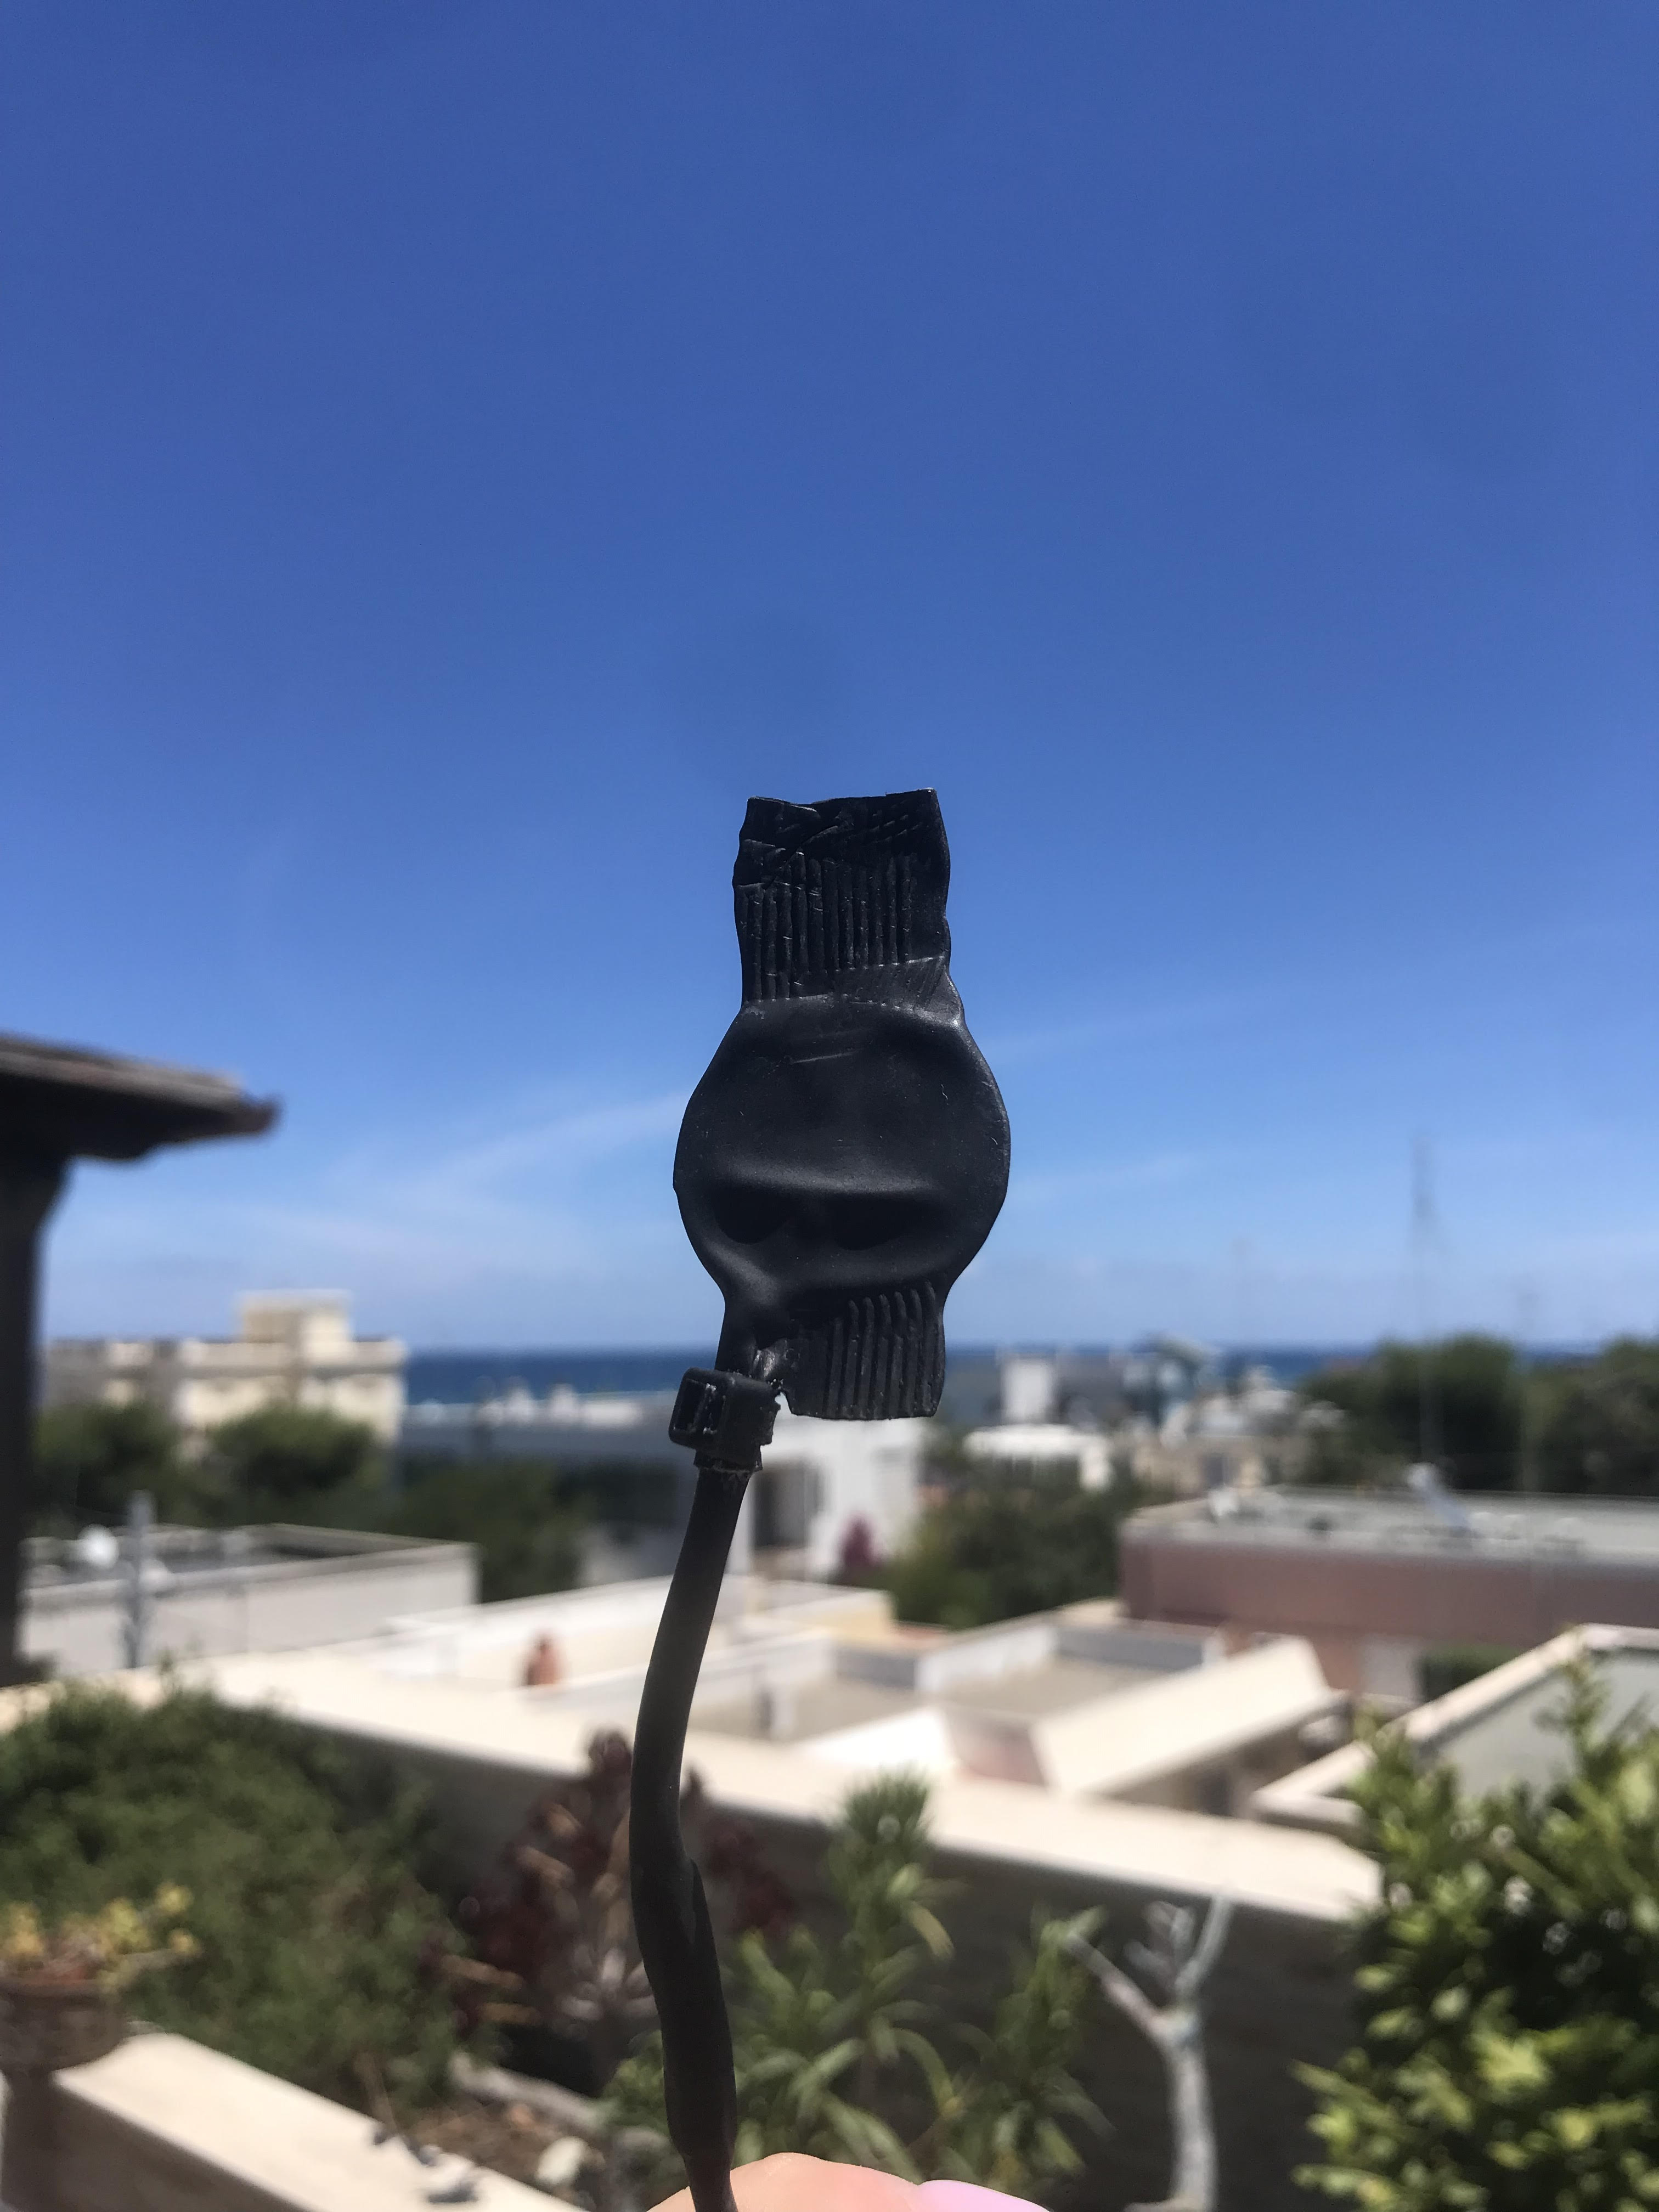
\includegraphics[width= .45\textwidth]{foto-idro}
\caption{Idrofono realizzato con trasduttori piezoelettrici}
\end{figure}

I due piezoelettrici sono stati bilanciati , positivamente e negativamente, per poi essere collegati all'interno del cavo XLR, e isolati con della plastica, proprio per utilizzarlo nell'immersione. 
L' idrofono DIY (do it yourself), è stato poi sottoposto a delle registrazioni in mare. 

Le registrazioni sono state eseguite in due luoghi differenti, Bari Santo Spirito e Molfetta. %\ref{Fig:recsspirito, Fig:recmilitari}

Nel primo caso, le riprese effettuate hanno riscontrato suoni e rumori, provenienti da motori di barche, rigetto di reti; 
La maggior parte delle registrazioni hanno ripreso rumori di fondo generali, dovuti al materiale con cui è stato costruito l'idrofono.

Nel secondo caso, le registrazioni alla profondità di 20mt, non hanno riscontrato particolare attenzione, rumori molto bassi o quasi indefinibili. 

\begin{figure}[h]
\centering
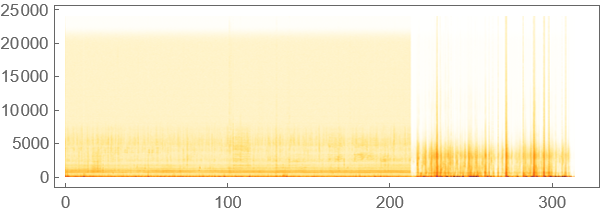
\includegraphics[width= .45\textwidth]{164431sspiritoporto}
\caption{Registrazione Porto S.Spirito}
\label{recsspirito}
\end{figure}

\begin{figure}[h]
\centering
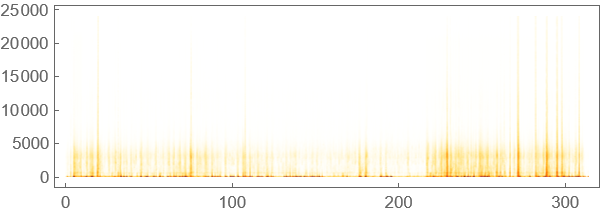
\includegraphics[width=.45\textwidth]{173608ZonaMilitarizzata}
\caption{Registrazione Zona Militarizzata}
\label{recmilitari}
\end{figure}

Proprio da questi esempi, l'utilizzo di un idrofono professionale avrebbe dato sicuramente una maggiore affidabilità a quello che è tutt'oggi l'obiettivo della ricerca. 

Cosa davvero provoca l'inquinamento acustico? Come il rumore contribuiscea definire inquinato il nostro mare?
Nell'immaginario collettivo, spesso l'ambiente subacqueo è totalmente privo di suoni, ma nella realtà non è così. Il mondo sottomarino è tutt'altro che silenzioso, e basta immergere la testa sott'acqua qualche secondo, per scoprirlo.

Nel linguaggio comune si parla di "rumore subacqueo", ma ciò che percepiamo, anche quando semplicemente nuotiamo in apnea, non è un singolo rumore, bensì la somma di una miriade di suoni. Sono i suoni prodotti dai numerosi organismi marini, i suoni originati dagli agenti atmosferici come il rumore delle onde e del vento, che si uniscono a loro volta ai rumori generati dalle attività umane, in certi casi particolarmente invasivi.

Per questo è più corretto parlare di "clima acustico subacqueo". 

L’ambiente marino consente al suono di percorrere notevoli distanze, nell’ordine di 1500 metri in un secondo, e ciò facilita la trasmissione, oltre che di suoni biologici, anche di tutta una vasta gamma di rumori, tra cui quelli di origine antropica, riguardo ai quali la comunità scientifica muove una sempre maggiore attenzione. Questi suoni, infatti, non interferiscono unicamente con le capacità sensoriali degli animali e la loro possibilità di comunicare, ma potrebbero anche avere una gamma più estesa di effetti, dalla morte immediata allo spostamento da abituali siti di foraggiamento ed anche di alterazione del rapporto preda/predatore o dei comportamenti riproduttivi e di orientamento. 

La Commissione Europea definisce l’inquinamento acustico sottomarino come “l’introduzione intenzionale o accidentale di energia acustica nella colonna d’acqua, da fonti puntuali o diffuse”.

Viste le scarse conoscenze specifiche sui suoi potenziali effetti si applica il "principio precauzionale" secondo cui l’assenza di certezza scientifica, qualora sussista il pericolo di danni gravi o irreversibili, non esonera gli Stati dal dovere di predisporre misure efficaci per evitare il degrado ambientale.

Per il monitoraggio del rumore subacqueo vengono presi in considerazione due indicatori:

\begin{itemize}
\item i suoni impulsivi, causati principalmente da attività esplorative a fini estrattivi e l’installazione di pali per la costruzione di piattaforme e stazioni eoliche
\item i suoni continui, generati principalmente dal trasporto marittimo
\end{itemize}

Grazie all'arpa FVG, sono riuscita ad avere contatti con MARITIME TECHNOLOGY CLUSTER FVG , Il punto di riferimento per il settore delle tecnologie marittime nel Friuli Venezia Giulia,un insieme di imprese, università, centri di ricerca, enti di formazione, il quale mi ha consigliato di contattare l'Istituto Nazionale di Oceanografia e di Geofisica Sperimentale nella provincia di Trieste. 

Grazie alla dott.ssa Tinivella, docente della sezione di Geofisica, ho avuto contatti con il CIBRA “Centro Interdisciplinare di Bioacustica”. 

Il CIBRA nasce nel 1989 come “Centro Interdisciplinare di Bioacustica” grazie al Professor Mario Pavan (1918-2003), allora Direttore dell'Istituto di Entomologia, e al Magnifico Rettore Roberto Schmid. 

Il Centro nasce sulle esperienze del Laboratorio di Bioacustica numerica avviato nove anni prima nell’ambito del lavoro di tesi del Dott. Gianni Pavan, e si è presto affermato come laboratorio all'avanguardia anche a livello internazionale nel settore della bioacustica e della nascente disciplina della Computational Bioacoustics. In seguito, il Centro cambia denominazione e diventa “Centro Interdisciplinare di Bioacustica e Ricerche Ambientali” per meglio indicare la valenza e le applicazioni della bioacustica nel settore ambientale, in particolare per il monitoraggio e la tutela della biodiversità.

Dalle prime ricerche strettamente di bioacustica sulle caratteristiche acustiche di singole specie, terrestri e marine, si passa a ricerche di più ampio respiro che si avvicinano ai temi dell'ecologia acustica e dell'acustica ambientale, fino a partecipare alla nascita nel 2014 di una nuova disciplina, l’Ecoacustica, che coniuga appunto bioacustica ed ecologia, e alla fondazione della International Ecoacoustic Society.

Negli ultimi anni, anche a causa dei costi elevati nel mantenere ricerche in mare, l'attenzione del CIBRA si è spostata sulla bioacustica e sull’ecoacustica come strumenti di monitoraggio ambientale terrestre e marino con la rivalutazione del concetto di Paesaggio Sonoro, tema talvolta borderline rispetto al tradizionale approccio scientifico.

il dott. Claudio Fossati Docente dell'Università di Pavia, specializzato nella ricerca del rumore del fondale marino, ha contribuito e collaborato alla ricerca di questo argomento, consegnandomi dati significativi, registrazioni provenienti dal mare della Puglia, che andremo in seguito ad analizzare. 

\section{2022: IronSolar - La costa pugliese fra i comuni di Melendugno e Brindisi} 
Nel 2022 il Dott.Fossati insieme a, Michele Manghi e Gianni Pavan, hanno realizzato uno studio sul prospetto del rumore inerente alla baseline di inquinamento acustico basato su impianti eolici. 
Il CIBRA e il NAUTA, collaborano con entità civili e militari per salvaguardare il rumore subaqueo di orgine antropica, lo studio del suo possibile impatto, e della sua conseguente mitigazione. 
Per quanto sia oggi relativamente facile reperire sistemi di raccolta e registrazione dei segnali acustici subacquei, la complessa dinamica e le caratteristiche del suono al di sotto della superficie del mare rendono il compito di documentare e descrivere i suoni sott’acqua estremamente delicato. 
Ancor più se il segnale raccolto deve essere utilizzato per estrarre misure di rumore univoche, come in questo caso. 
Anche in tema di analisi dei dati è necessaria una solida esperienza fondamentale per eseguire corrette misure di livelli e individuare e interpretare i segnali biologici.
Le uscite in mare per la raccolta dei dati nel lavoro illustratomi dal Dott.Fossati sono state svolte a bordo di una piccola imbarcazione di servizio a motore con porto di ormeggio a sud di Brindisi. 
Il porto base per la gestione delle operazioni è stato quello di San Foca, a poca distanza da Melendugno. 
La campagna di misure si è svolta nel mese di Novembre 2022. 

\subsection{Baseline acustica, materiali, metodi} 
Fondamentale e propedeutica a qualsiasi valutazione di impatto è la conoscenza della baseline acustica esistente. 
Dal punto di vista acustico, nel caso esaminato, essa si compone fondamentalmente di due componenti: il rumore ambiente, o panorama acustico, e una valutazione dei mammiferi. 
Sia i dati acustici che le osservazioni in superficie concorrono a evidenziare le caratteristiche dell’area, e permettono di definire e prevedere le componenti del rumore presente e futuro (associato al campo eolico) per bande di frequenza, 
sovrapponendole poi con quelle utilizzate in natura, dalle specie presenti, per una corretta valutazione di impatto. 

La scelta del setup strumentale è stata eseguita conformemente alle caratteristiche dell'ambiente oggetto di studio. 
Profondità, correnti e il tipo di fondale influenzano infatti la scelta dello strumento e il tipo di ancoraggio più adatti, insieme ad altri parametri tipo durata della deposizione, traffico navale, pesca ecc. 
Data la necessità di eseguire misure calibrate rappresentative dell'intensità del rumore presente, è fondamentale evitare qualsiasi tipo di interferenza acustica eventualmente generata dal sistema di deposizione, dall’ancoraggio e dall’imbarcazione di servizio. 
Per la campagna in oggetto si è scelto di utilizzare registratori acustici autonomi, descritti più avanti, adottando un sistema di ancoraggio composto da doppia zavorra separate da qualche metro di cima. 
La prima zavorra viene fissata a una breve cima immersa su cui sono vincolati registratore e galleggiante di profondità, la seconda zavorra, più pesante, è fissata alla linea fino alla superficie dove si trovano i galleggianti di segnalazione, la luce intermittente, un riflettore radar e un transponder satellitare. 

Questo sistema di deposizione a J permette di isolare il sensore dai movimenti della cima che raggiunge la superficie.
Il programma ha previsto la raccolta di una sessione di registrazione di almeno 24 ore in quattro punti diversi e rappresentativi dell’area di intervento. 

Tutte le registrazioni sono state raccolte con metodo identico e successivamente analizzate. 
La strumentazione impiegata e i protocolli sono stati standardizzati in modo da rendere il lavoro di analisi e i conseguenti risultati omogenei e confrontabili fra loro.
In particolare, per le sessioni di registrazione, sono stati impiegati registratori calibrati di due tipi: {\bfseries Soundtrap ST300STD e uRec384k 22D}.
Infine le registrazioni raccolte sono state poi analizzate in seguito. 

\subsection{Analisi Acustica}
L’analisi acustica delle registrazioni è stata focalizzata su due aspetti:

\begin{itemize}
\item misure di rumore con misura dei parametri (descrizione quantitativa) 
\item individuazione di segnali biologici e antropici (descrizione qualitativa)
\end{itemize} 

Il primo passo è stato quello qualitativo, per avere una visione d’insieme del panorama acustico subacqueo rilevato.
E' stato utilizzato il software di SEAPro brevettato da Giovanni Pavan, che ha collaborato in questo progetto. 
Le registrazioni sono state analizzate grazie allo spettrogramma professionale del software che ha rilevato rumori di cetacei ma anche di imbarcazioni. 
Sono stati rilevati degli Alfeidi, un click che è stato rilevato sulle prime 24 ore di raccolta delle registrazioni. Sono piccoli crostacei decapodi, lunghi pochi millimetri, con la peculiare caratteristica di emettere click molto intensi, malgrado le dimensioni ridotte degli individui, e a banda larga, attraverso lo schiocco di una chela ipertrofica. %inserire spettrogramma? 
Il “rumore” generato da questi piccoli crostacei costituisce una componente non trascurabile del panorama acustico subacqueo soprattutto alle frequenze medio alte, rendendo molto difficile evidenziare i click di ecolocalizzazione distintivi dei delfini.
I delfini registrati, sono stati evidanziati dall' accentuazione sulle alte frequenze, ben oltre la soglia udibile dagli esseri umani. 
L'analisi qualitativa effettuata dal software SEAPro ha evidanziato anche macroeventi che evidenziano il passaggio di una nave nelle vicinanze, ma anche di far emergere, al verificarsi delle adeguate condizioni (es. rapporto segnale rumore) 
serie di click di delfini nel contesto acusticamente complesso che caratterizza queste registrazioni. 
Il picco del segnale dei delfini, è in concomitanza con il passaggio di un'imbarcazione. 
Da numerose osservazioni fatte in precedenti studi in Adriatico, ma valide anche per gli altri mari d’Italia e non solo, i tursiopi hanno imparato a seguire i pescherecci, specialmente quelli a strascico, per predare il contenuto delle reti. 
Il comportamento è molto diffuso ed espone gli animali a diversi rischi. Non ultimo, quello dell’esposizione cronica al rumore del peschereccio impegnato nelle operazioni di traina.

Sono stati anche registrati fischi, tipicamente associati a comportamenti sociali. 

I segnali acustici maggiormente rappresentati, però, sono stati quelli associati al traffico navale. 
L’area è risultata essere particolarmente trafficata, sia per la presenza di pescherecci, che per la “vicinanza” di una delle rotte di accesso al mar Adriatico e ai suoi porti.
L’immagine che segue è una rappresentazione dove l’immagine di base è tratta dal sito Marinetraffic.com. 
Rappresenta, con un indice di colore, il traffico cumulato nel 2021 nella zona in cui si dovrà realizzare l’impianto. 
Per facilitare la lettura è stata sovrapposta la mappa progettuale per il campo eolico. 
Risulta chiaramente come l’impianto, e quindi l’area di indagine di questo studio, si trovi in un’area di transito importante. 

\begin{figure}[h]
\centering 
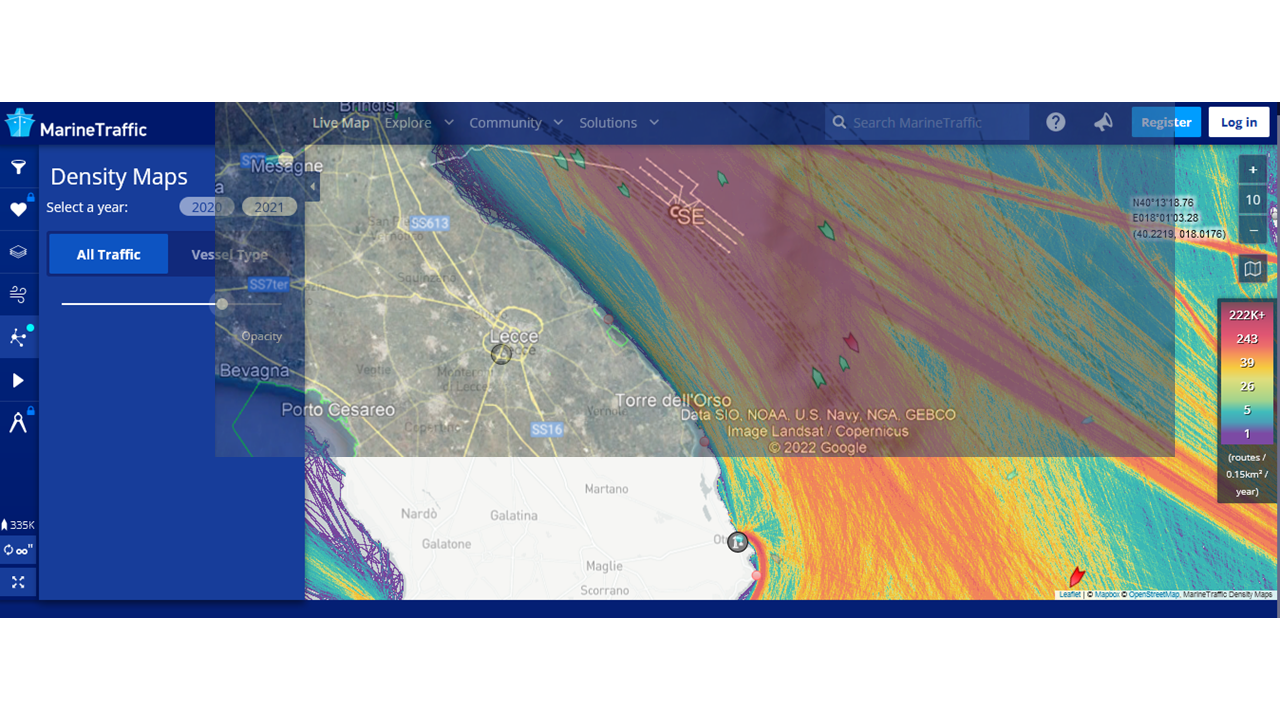
\includegraphics[width=.5\textwidth]{marinetraffic.com}
\caption{Estratto da Marinetraffic.com. Mappa cumulativa del traffico del 2021. In rosso le aree più trafficate}
\end{figure} 

La grafica delle rotte navali ha una chiara ripercussione sull’andamento del rumore subacqueo.

\subsection{Risultati}
 
Riassumendo i dati dell’analisi acustica qualitativa svolta, si possono evidenziare i seguenti risultati: 
\begin{itemize} 
\item Sono state eseguite 4 stazioni di campionamento da 24 ore. È stato possibile evidenziare la presenza di click di alfeidi per la totalità del periodo di osservazione, senza variazioni significative fra giorno e notte. 
\item I click di delfini sono stati evidenziati 2 volte, ma è probabile una presenza maggiore, impossibile da evidenziare dato il contesto acustico presente (click di alfeidi). 
\item Interessante da notare, e sottolineare, come delle 2 presenze di Cetacei accertate, una sia certamente associata alla presenza di un peschereccio. 
\item Come osservato in numerose altre campagne di avvistamento, i tursiopi hanno sviluppato l’abitudine di seguire gli strascichi per alimentarsi. 
Le registrazioni hanno confermato, anche acusticamente e anche per questo contesto, questo comportamento. 
\end{itemize} 

A completamento dell’analisi acustica qualitativa, durante la navigazione nell’area per la deposizione e il recupero degli strumenti, sono anche state condotte osservazioni visive. 
Nei primi giorni il meteo non era favorevole, in seguito all'avvistamenteo di altri animali, il meteo è stato a favore del recupero degli idrofoni. 

L'analisi acustica quantitativa è stata eseguita utilizzando due software: 
\begin{itemize}
\item DbWav %{\href {https://au.marshallday.com/innovation/software/dbwav/}{\DbWav}.
\item VSLM Virtual Sound Level Meter %{\href {https://doi.org/10.1121/1.5036041}{\VSLM}. 
\end{itemize} 

Il primo è in grado di produrre spettri compatti con relative misure di interi periodi di 24 ore
Il secondo è stato invece usato per caratterizzare segmenti di registrazioni con particolare significato come momenti di silenzio o periodi di rumore intenso, nonché per misure estensive (es calcoli LEQ - Livelli Equivalenti).

Nell’analisi condotta non si è applicata nessuna pesatura (curva di correzione) in modo da poter avere una baseline acustica su cui confrontare l’apporto del campo eolico. 
I livelli sono pertanto quelli reali.

I valori raccolti hanno riscontrato un evidente rumore associato principalmente al traffico navale(122db). 
Per completezza si riportano i grafici relativi alle ore di massima e minima intensità. il LEQ mediato su 60 secondi 

\begin{figure}[h]
\centering
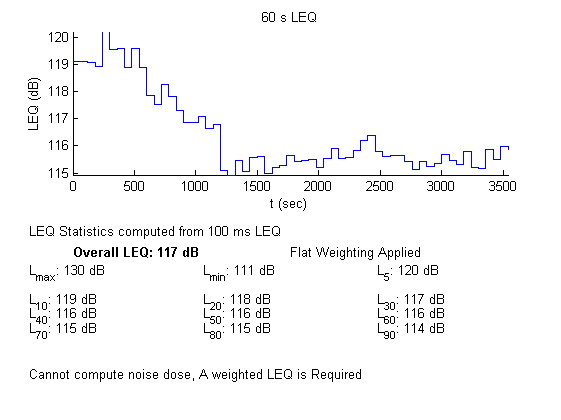
\includegraphics[width=.45\textwidth]{LEQ-di-un-segmento-silenzioso}
\caption{LEQ di un segmento “silenzioso”}
\end{figure}

Dopo il passaggio relativamente veloce di un’imbarcazione, segue un periodo di silenzio, pur sempre compreso fra 115 e 116 dB, valori comunque alti per un ambiente naturale ben conservato.

Il grafico seguente rappresenta invece la distribuzione del rumore in bande di terzi d’ottava per le frequenze fino a 18kHz. 
La rappresentazione delle frequenze, sulle ascisse, pone in risalto le frequenze più basse. 
Questo tipo di grafico permette di valutare la distribuzione in frequenza dei livelli di segnale.

\begin{figure}[h]
\centering
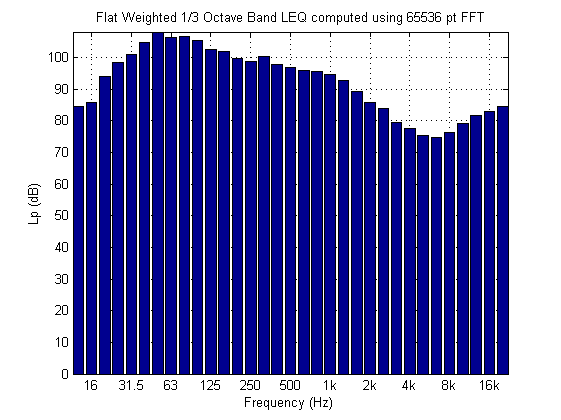
\includegraphics[width=.45\textwidth]{Bande-in-terzi-d'ottava}
\caption{Bande in terzi d’ottava}
\end{figure}

Si può notare come tutta la banda compresa fra i 30Hz circa e i 2 kHz contenga la maggior parte dell’energia presente. 
Questa è la tipica impronta del rumore associato al traffico navale. 
Anche il grafico PSD (Power Spectral Density) evidenzia chiaramente lo stesso andamento.

\begin{figure}[h]
\centering
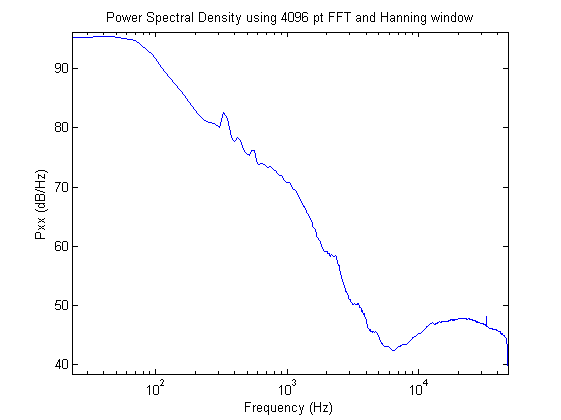
\includegraphics[width=.45\textwidth]{Grafico-Power-Spectral-Density}
\caption{Grafico Power Spectral Density}
\end{figure}

Le stesse analisi, con gli stessi parametri, sono state calcolate per l’ora con il livello LEQ più intenso 

\begin{figure}[h]
\centering
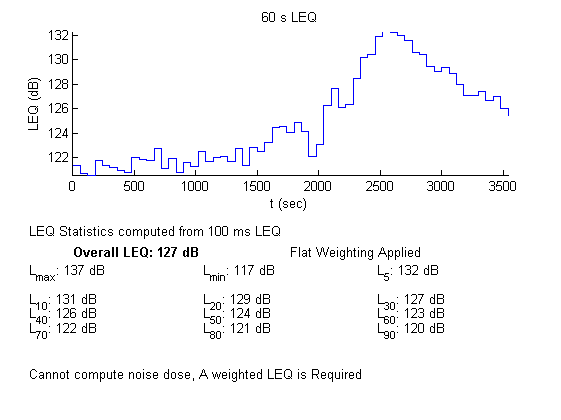
\includegraphics[width=.45\textwidth]{LEQ-rumoroso}
\caption{LEQ di un segmento significativamente rumoroso}
\end{figure}

Su un rumore di fondo già elevato (sopra i 120dB) si inserisce il passaggio di una nave particolarmente rumorosa (picco massimo a 137dB intorno al secondo 2600). 
Il grafico a bande di terzi d’ottava e la PSD - Power Spectral Density evidenziano che, oltre alla elevata intensità, in questo caso tutte le bande di frequenza sono interessate. 

\begin{figure}[h]
\centering
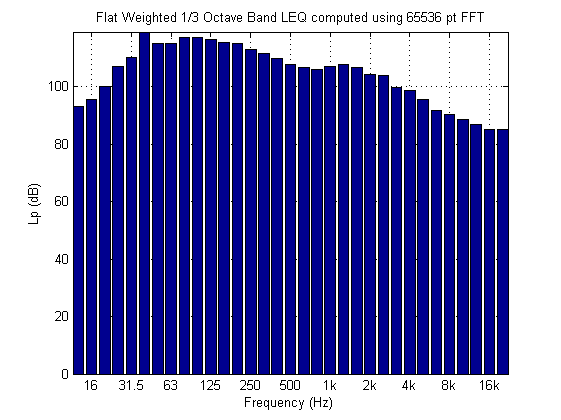
\includegraphics[width=.45\textwidth]{Bandi-in-terzi-d'ottava-rumorose}
\caption{Bande in terzi d’ottava, segmento rumoroso con componente rumore navale a tutte le frequenze}
\end{figure}

\begin{figure}[h]
\centering
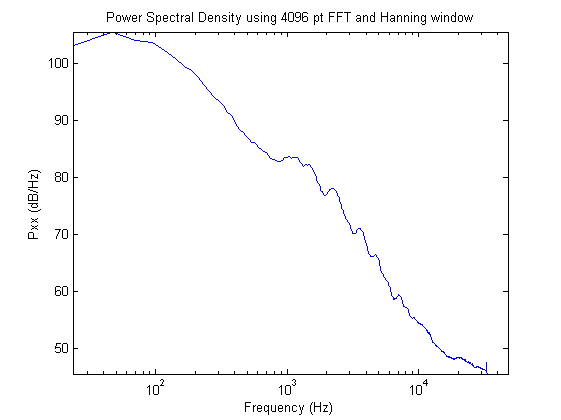
\includegraphics[width=.45\textwidth]{psd-rumoroso}
\caption{PSD dello stesso segmento precendente}
\end{figure}















